\section{Problem 2}
State space representation of a 2-mass system.

For the following mechanical system, there is one input, $f$, and two outputs: the position of the first mass, $z_1$, and the distance between the masses, $z_1 - z_2$.

\begin{figure}[htp]
    \centering
    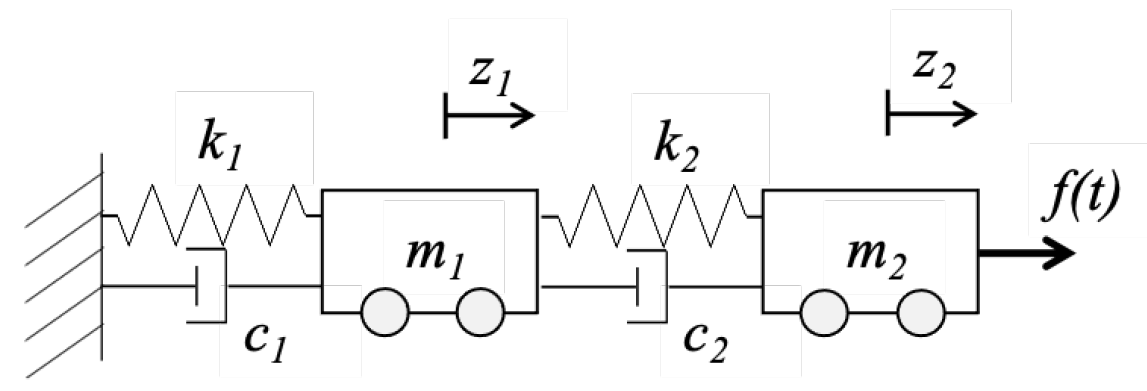
\includegraphics[width=15cm]{images/Q2.png}
\end{figure}

\subsection{a)}
Write the state equation, $\dot{x}=Ax+Bu$, where $x$ is a state vector that you choose, $A$ is the system matrix, $B$ is the input matrix, and $u$ is the input.
\subsubsection{solution}

First we identify all energy storage elements:

\begin{table}[ht]
    \centering
    \begin{tabular}{c | c}
        Energy Storage Elements & State variable
        \\
        \hline
        $m_1$ (Kinetic) & $\dot{z_1}$ \\
        $m_2$ (Kinetic) & $\dot{z_2}$ \\
        $k_1$ (Potential) & $z_1$ \\
        $k_2$ (Potential) & $z_2 - z_1$
    \end{tabular}
\end{table}

From all energy storage elements we define the state vector: $\textbf{x} = 
\begin{bmatrix}
    x_1\\
    x_2\\ 
    x_3\\ 
    x_4
\end{bmatrix} = 
\begin{bmatrix}
    z_1\\
    z_2 - z_1\\ 
    \dot{z_1}\\ 
    \dot{z_2}
\end{bmatrix}$, and input $u = f$

Draw FBD to analyze system dynamics: 
\begin{figure}[htp]
    \centering
    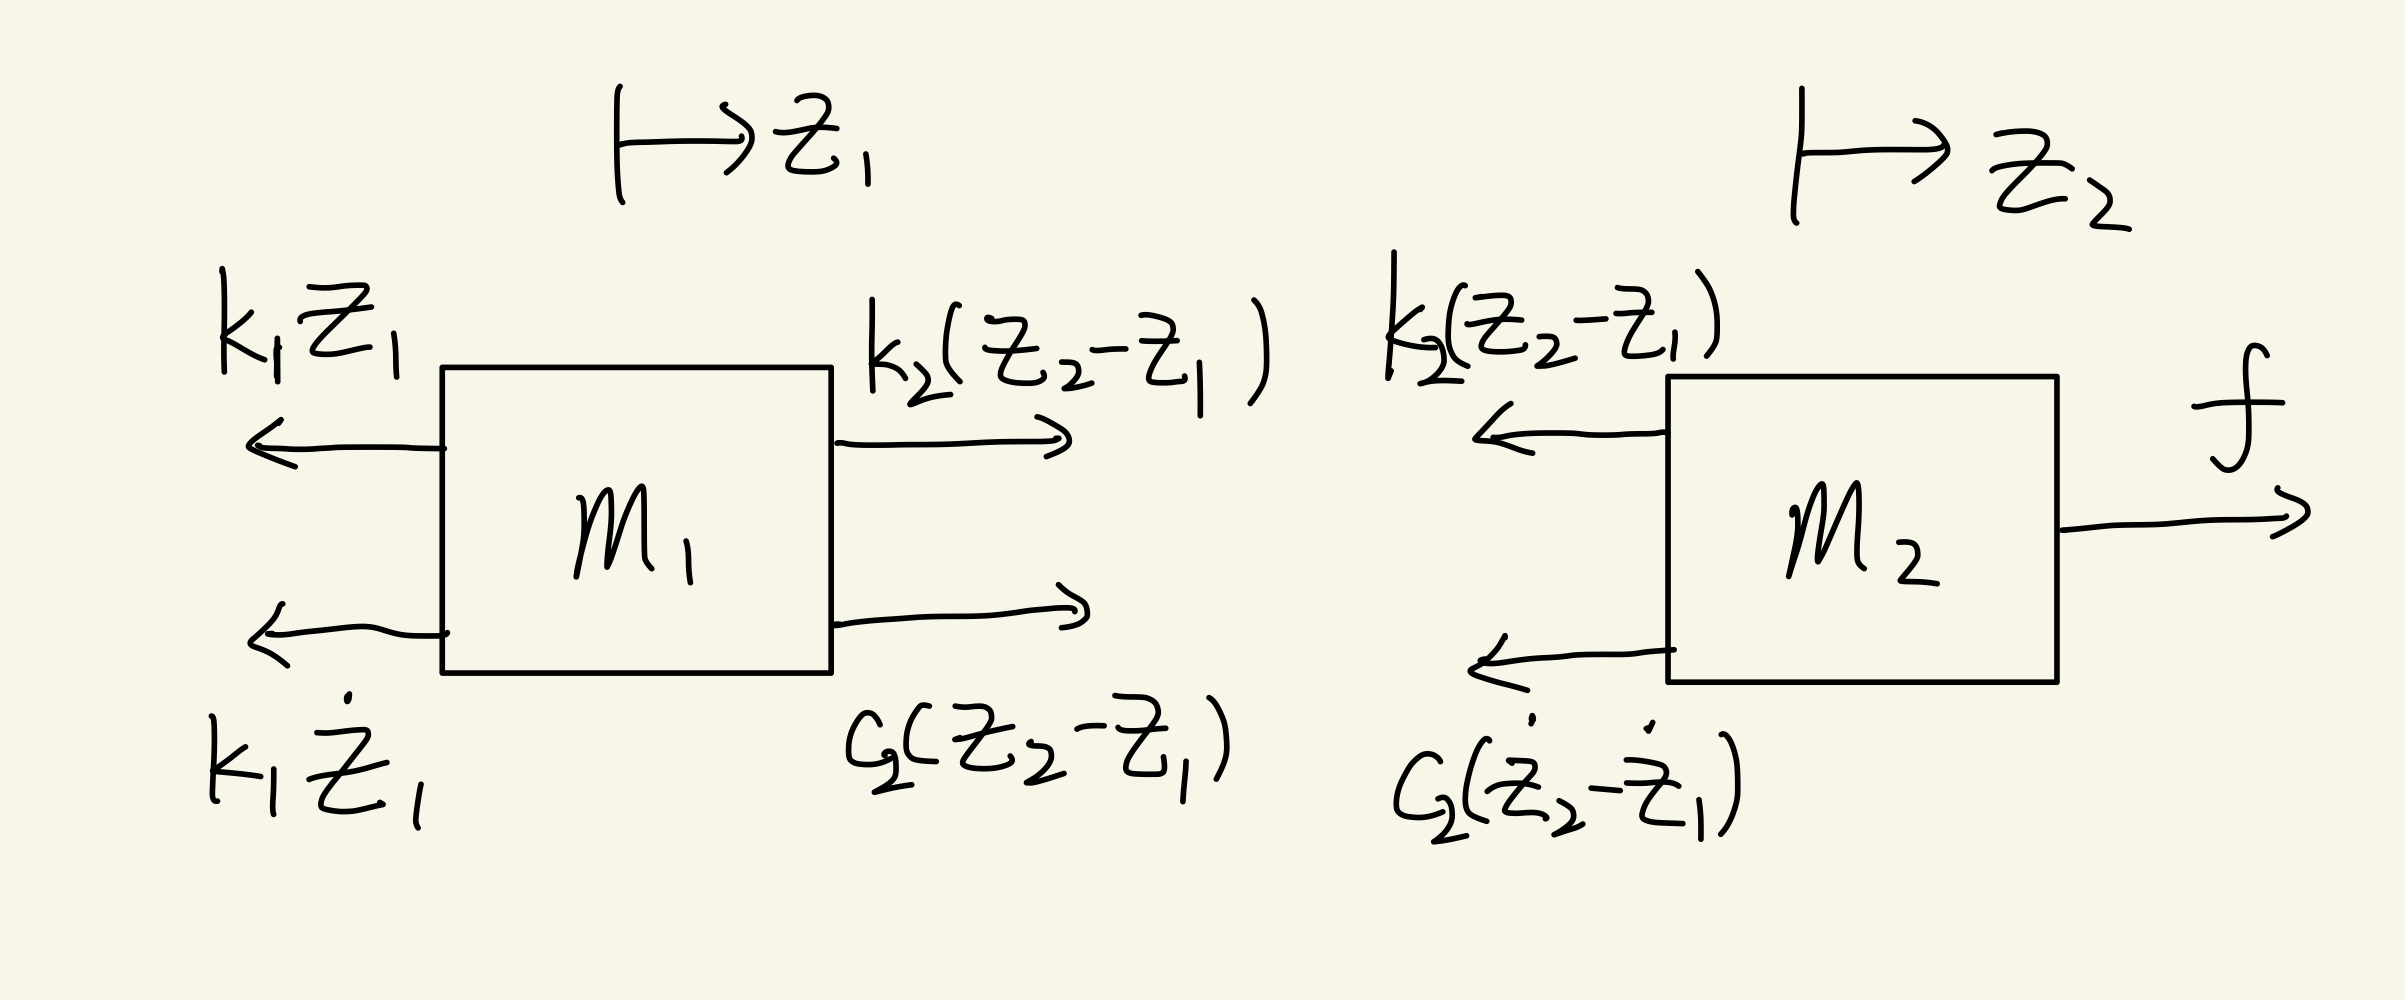
\includegraphics[width=10cm]{images/Q2_FBD.png}
    \caption{Free body diagram}
    \label{fig:Q2FBD}
\end{figure}

We get the following dynamic equations:

$\left\{
    \begin{array}{lr}
    m_1\ddot{z_1} = k_2(z_2 - z_1) + c_2(\dot{z_2} - \dot{z_1}) - k_1z_1 -c_1\dot{z_1}\\
    m_2\ddot{z_2} = f - k_2(z_2 - z_1) - c_2(\dot{z_2} - \dot{z_1})\\
    \end{array}
\right.$ 

$\Rightarrow $
$\left\{
    \begin{array}{lr}
    \dot{x_1} = \dot{z_1} \\ 
    \dot{x_2} = \dot{z_2} - \dot{z_1}\\
    \dot{x_3} = \ddot{z_1} = \frac{k_2}{m_1} (z_2 - z_1) + \frac{c_2}{m_1}(\dot{z_2} - \dot{z_1}) - \frac{k_1}{m_1}z_1 -\frac{c_1}{m_1}\dot{z_1}\\
    \dot{x_4} = \ddot{z_2} = \frac{f}{m_2} - \frac{k_2}{m_2}(z_2 - z_1) - \frac{c_2}{m_2}(\dot{z_2} - \dot{z_1})\\
    \end{array}
\right.$

$\Rightarrow $
$\left\{
    \begin{array}{lr}
    \dot{x_1} = 0x_1 + 0x_2 + x_3 + 0x_4 + 0u \\ 
    \dot{x_2} = 0x_1 + 0x_2 + (-1)x_3 + x_4 + 0u \\
    \dot{x_3} = - \frac{k_1}{m_1}x_1 + \frac{k_2}{m_1} x_2 - \frac{c_1+c_2}{m_1}x_3 + \frac{c_2}{m_1}x_4 + 0u\\
    \dot{x_4} = 0x_1 - \frac{k_2}{m_2}x_2 + \frac{c_2}{m_2}x_3 - \frac{c_2}{m_2}x_4 + \frac{1}{m_2}u\\
    \end{array}
\right.$

We can write the state space equation as:
\begin{equation}
    \dot{\textbf{x}} =
        \begin{bmatrix}
        0                & 0                & 1                    & 0 \\
        0                & 0                & -1                   & 1 \\ 
        -\frac{k_1}{m_1} & \frac{k_2}{m_1}  & -\frac{c_1+c_2}{m_1} & \frac{c_2}{m_1}  \\ 
        0                & -\frac{k_2}{m_2} & \frac{c_2}{m_2}      & -\frac{c_2}{m_2}
    \end{bmatrix}
    \textbf{x} + 
    \begin{bmatrix}
        0\\
        0\\ 
        0\\ 
        \frac{1}{m_2}
    \end{bmatrix}
    u
\end{equation}

\subsection{b)}
Write the output equation, $y = Cx + Du$.
\subsubsection{solution}
The output vector: $\textbf{y} = 
\begin{bmatrix}
    z_1\\
    z_1 - z_2
\end{bmatrix} = 
\begin{bmatrix}
    x_1\\
    - x_2
\end{bmatrix}$, thus: 

\begin{equation}
    \dot{\textbf{y}} =
        \begin{bmatrix}
        1 & 0  & 0 & 0 \\
        0 & -1 & 0 & 0 \\ 
    \end{bmatrix}
    \textbf{x} + 
    \begin{bmatrix}
        0\\
        0
    \end{bmatrix}
    u
\end{equation}

\pagebreak